% This is figure 1. It contains model and results validating the model.
\RequirePackage{luatex85,shellesc}
\documentclass[multi=false,crop,class=../pnas-new]{standalone}
\usepackage{pgfplots}
\pgfplotsset{compat=newest}

\usepackage{siunitx}
\usetikzlibrary{positioning,calc}
\usepgfplotslibrary{units}
\usepackage{opensans}
\usepackage{mathpazo}

\begin{document}

\edef\figW{15}
\edef\plotH{3}
\pgfmathsetmacro{\colW}{0.5*\figW}
\pgfmathsetmacro{\plotW}{0.9*\colW}
\pgfmathsetmacro{\VGapBetweenAxis}{-15mm}
\renewcommand\familydefault{\sfdefault}
\newcommand\LABELAXIS[2]{\node[above left=of #1.north west,yshift=-9mm] (#1.label) {\bf #2};}

\pgfplotsset{
    , xtick align=center
    , ytick align=center
    , unit markings=parenthesis
    , legend style={fill=none,draw=none,font=\footnotesize}
    , axis lines=left
    , axis line style={-}
    , title style={yshift=-2mm}
    , label style={font=\small}
    , tick label style={font=\scriptsize}
}

\pgfmathsetmacro{\plotAW}{0.35*\figW}
\pgfmathsetmacro{\plotBW}{0.55*\figW}

\begin{tikzpicture}[scale=1, every node/.style={} ]

    \node[label=north west:{\bf A}] (reac)  at (0,0)
    {
        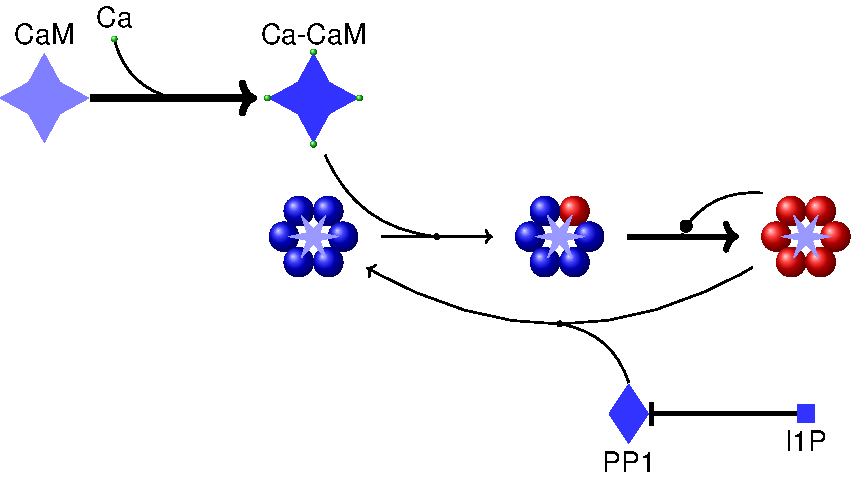
\includegraphics[width=\plotAW cm]{./camkii_pp1_switch_level1_detail.pdf} 
    };

    \node[below=of reac,yshift=1cm] (su) {
        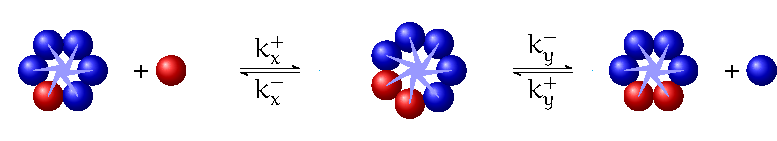
\includegraphics[width=\plotAW cm]{./camkii_subunit_exchage.pdf}
    };

    \begin{axis}[ name=B
        , at=(reac.north east), anchor=north west, xshift=15mm
        , width=\plotBW cm, height=\plotH cm
        , enlarge y limits
        , ytick={0,1}
        , yticklabels={OFF,ON}
        , title={Number of CaMKII=15}
        , xlabel=Time, x unit=day
        ]
        \addplot [color=blue] gnuplot [ raw gnuplot ] {
            plot "./_data/camkii_35_long.dat" every 50
            using (column("time")/86400/30):(column("CaMKII*")/35)
        };
    \end{axis}
    \LABELAXIS{B}{B}

    \begin{semilogyaxis}[ name=C
       , at=(B.south west), anchor=north west
       , yshift = \VGapBetweenAxis
       , xlabel = Number of CaMKII (x)
       , width = 0.55*\plotBW cm
       , ylabel = Stability
       , legend pos=outer north east
       , enlargelimits
       , grid
       ]
       \addplot[only marks, blue, thick, mark size=2pt,mark=o] table
           [col sep=comma,x=CaMKII,y=CramerTime] {./_data/switch_stability.csv};
       \addplot [domain=5:40, blue, very thick, smooth, solid, no markers] {exp((x-8)/4.2)};
       \legend{Simulation data,fit $e^{\left(\frac{x-8}{4.2}\right)}$}
    \end{semilogyaxis}
    \LABELAXIS{C}{C}
\end{tikzpicture}
\end{document}
